\documentclass[12pt]{article}
\usepackage[left=1cm, right=1cm, top=2cm,bottom=1.5cm]{geometry} 

\usepackage[parfill]{parskip}
\usepackage[utf8]{inputenc}
\usepackage[T2A]{fontenc}
\usepackage[russian]{babel}
\usepackage{enumitem}
\usepackage[normalem]{ulem}
\usepackage{amsfonts, amsmath, amsthm, amssymb, mathtools,xcolor,accents}
\usepackage{blkarray}

\usepackage{tabularx}
\usepackage{hhline}

\usepackage{accents}
\usepackage{fancyhdr}
\pagestyle{fancy}
\renewcommand{\headrulewidth}{1.5pt}
\renewcommand{\footrulewidth}{1pt}

\usepackage{graphicx}
\usepackage[figurename=Рис.]{caption}
\usepackage{subcaption}
\usepackage{float}

%%Наименование папки откуда забирать изображения
\graphicspath{ {./images/} }

%%Изменение формата для ввода доказательства
\renewcommand{\proofname}{$\square$  \nopunct}
\renewcommand\qedsymbol{$\blacksquare$}

%%Изменение отступа на таблицах
\addto\captionsrussian{%
	\renewcommand{\proofname}{$\square$ \nopunct}%
}
%% Римские цифры
\newcommand{\RN}[1]{%
	\textup{\uppercase\expandafter{\romannumeral#1}}%
}

%% Для удобства записи
\newcommand{\MR}{\mathbb{R}}
\newcommand{\MC}{\mathbb{C}}
\newcommand{\MQ}{\mathbb{Q}}
\newcommand{\MN}{\mathbb{N}}
\newcommand{\MZ}{\mathbb{Z}}
\newcommand{\MTB}{\mathbb{T}}
\newcommand{\MTI}{\mathbb{I}}
\newcommand{\MI}{\mathrm{I}}
\newcommand{\MCI}{\mathcal{I}}
\newcommand{\MCR}{\mathcal{R}}
\newcommand{\MJ}{\mathrm{J}}
\newcommand{\MH}{\mathrm{H}}
\newcommand{\MT}{\mathrm{T}}
\newcommand{\MU}{\mathcal{U}}
\newcommand{\MV}{\mathcal{V}}
\newcommand{\MA}{\mathcal{A}}
\newcommand{\MB}{\mathcal{B}}
\newcommand{\MF}{\mathcal{F}}
\newcommand{\ME}{\mathcal{E}}
\newcommand{\MW}{\mathcal{W}}
\newcommand{\ML}{\mathcal{L}}
\newcommand{\MM}{\mathcal{M}}
\newcommand{\MP}{\mathcal{P}}
\newcommand{\VN}{\varnothing}
\newcommand{\VE}{\varepsilon}
\newcommand{\dx}{\, dx}
\newcommand{\dy}{\, dy}
\newcommand{\dz}{\, dz}
\newcommand{\dd}{\, d}


\theoremstyle{definition}
\newtheorem{defn}{Опр:}
\newtheorem{rem}{Rm:}
\newtheorem{prop}{Утв.}
\newtheorem{exrc}{Упр.}
\newtheorem{problem}{Задача}
\newtheorem{lemma}{Лемма}
\newtheorem{theorem}{Теорема}
\newtheorem{corollary}{Следствие}

\newenvironment{cusdefn}[1]
{\renewcommand\thedefn{#1}\defn}
{\enddefn}

\DeclareRobustCommand{\divby}{%
	\mathrel{\text{\vbox{\baselineskip.65ex\lineskiplimit0pt\hbox{.}\hbox{.}\hbox{.}}}}%
}
\DeclareRobustCommand{\ndivby}{\mkern-1mu\not\mathrel{\mkern4.5mu\divby}\mkern1mu}


%Короткий минус
\DeclareMathSymbol{\SMN}{\mathbin}{AMSa}{"39}
%Длинная шапка
\newcommand{\overbar}[1]{\mkern 1.5mu\overline{\mkern-1.5mu#1\mkern-1.5mu}\mkern 1.5mu}
%Функция знака
\DeclareMathOperator{\sgn}{sgn}

%Функция ранга
\DeclareMathOperator{\rk}{\text{rk}}
\DeclareMathOperator{\diam}{\text{diam}}


%Обозначение константы
\DeclareMathOperator{\const}{\text{const}}

\DeclareMathOperator{\codim}{\text{codim}}

\DeclareMathOperator*{\dsum}{\displaystyle\sum}
\newcommand{\ddsum}[2]{\displaystyle\sum\limits_{#1}^{#2}}
\newcommand{\ddssum}[2]{\displaystyle\smashoperator{\sum\limits_{#1}^{#2}}}
\newcommand{\ddlsum}[2]{\displaystyle\smashoperator[l]{\sum\limits_{#1}^{#2}}}
\newcommand{\ddrsum}[2]{\displaystyle\smashoperator[r]{\sum\limits_{#1}^{#2}}}

%Интеграл в большом формате
\DeclareMathOperator{\dint}{\displaystyle\int}
\newcommand{\ddint}[2]{\displaystyle\int\limits_{#1}^{#2}}
\newcommand{\ssum}[1]{\displaystyle \sum\limits_{n=1}^{\infty}{#1}_n}

\newcommand{\smallerrel}[1]{\mathrel{\mathpalette\smallerrelaux{#1}}}
\newcommand{\smallerrelaux}[2]{\raisebox{.1ex}{\scalebox{.75}{$#1#2$}}}

\newcommand{\smallin}{\smallerrel{\in}}
\newcommand{\smallnotin}{\smallerrel{\notin}}

\newcommand*{\medcap}{\mathbin{\scalebox{1.25}{\ensuremath{\cap}}}}%
\newcommand*{\medcup}{\mathbin{\scalebox{1.25}{\ensuremath{\cup}}}}%

\makeatletter
\newcommand{\vast}{\bBigg@{3.5}}
\newcommand{\Vast}{\bBigg@{5}}
\makeatother

%Промежуточное значение для sup\inf, поскольку они имеют разную высоту
\newcommand{\newsup}{\mathop{\smash{\mathrm{sup}}}}
\newcommand{\newinf}{\mathop{\mathrm{inf}\vphantom{\mathrm{sup}}}}

%Скалярное произведение
\newcommand{\inner}[2]{\left\langle #1, #2 \right\rangle }
\newcommand{\linsp}[1]{\left\langle #1 \right\rangle }
\newcommand{\linmer}[2]{\left\langle #1 \vert #2\right\rangle }

%Подпись символов снизу
\newcommand{\ubar}[1]{\underaccent{\bar}{#1}}

%%Шапка для букв сверху
\newcommand{\wte}[1]{\widetilde{#1}}
\newcommand{\wht}[1]{\widehat{#1}}
\newcommand{\ovl}[1]{\overline{#1}}
\newcommand{\unl}[1]{\underline{#1}}


%%Трансформация Фурье
\newcommand{\fourt}[1]{\mathcal{F}\left(#1\right)}
\newcommand{\ifourt}[1]{\mathcal{F}^{-1}\left(#1\right)}

%%Символ вектора
\newcommand{\vecm}[1]{\overrightarrow{#1\,}}

%%Пространстов матриц
\newcommand{\matsq}[1]{\operatorname{Mat}_{#1}}
\newcommand{\mat}[2]{\operatorname{Mat}_{#1, #2}}

%Оператор для действ и мнимых чисел
\DeclareMathOperator{\IM}{\operatorname{Im}}
\DeclareMathOperator{\RE}{\operatorname{Re}}
\DeclareMathOperator{\li}{\operatorname{li}}
\DeclareMathOperator{\GL}{\operatorname{GL}}
\DeclareMathOperator{\SL}{\operatorname{SL}}
\DeclareMathOperator{\Char}{\operatorname{char}}
\DeclareMathOperator\Arg{Arg}
\DeclareMathOperator\ord{ord}

%Оператор для образа
\DeclareMathOperator{\Ima}{Im}

%Делимость чисел
\newcommand{\modn}[3]{#1 \equiv #2 \; (\bmod \; #3)}
\newcommand{\nmodn}[3]{#1 \not\equiv #2 \; (\bmod \; #3)}

%%Взятие в скобки, модули и норму
\newcommand{\parfit}[1]{\left( #1 \right)}
\newcommand{\modfit}[1]{\left| #1 \right|}
\newcommand{\sqparfit}[1]{\left\{ #1 \right\}}
\newcommand{\normfit}[1]{\left\| #1 \right\|}

%%Функция для обозначения равномерной сходимости по множеству
\newcommand{\uconv}[1]{\overset{#1}{\rightrightarrows}}
\newcommand{\uconvm}[2]{\overset{#1}{\underset{#2}{\rightrightarrows}}}

%% Функция для добавления круга сверху множества
\newcommand{\Circ}[1]{\accentset{\circ}{#1}}

%% Жирное подчеркивание
\newcommand{\buline}[1]{\textbf{\uline{#1}}}

%%Функция для обозначения нижнего и верхнего интегралов
\def\upint{\mathchoice%
	{\mkern13mu\overline{\vphantom{\intop}\mkern7mu}\mkern-20mu}%
	{\mkern7mu\overline{\vphantom{\intop}\mkern7mu}\mkern-14mu}%
	{\mkern7mu\overline{\vphantom{\intop}\mkern7mu}\mkern-14mu}%
	{\mkern7mu\overline{\vphantom{\intop}\mkern7mu}\mkern-14mu}%
	\int}
\def\lowint{\mkern3mu\underline{\vphantom{\intop}\mkern7mu}\mkern-10mu\int}

%%След матрицы
\DeclareMathOperator*{\tr}{tr}

\DeclareMathOperator*{\symdif}{\bigtriangleup}

% Верхние\нижние пределы
\DeclareMathOperator*\lowlim{\underline{lim}}
\DeclareMathOperator*\uplim{\overline{lim}}

\makeatletter
\renewcommand*\env@matrix[1][*\c@MaxMatrixCols c]{%
	\hskip -\arraycolsep
	\let\@ifnextchar\new@ifnextchar
	\array{#1}}
\makeatother


%% Переопределение функции хи, чтобы выглядела более приятно
\makeatletter
\@ifdefinable\@latex@chi{\let\@latex@chi\chi}
\renewcommand*\chi{{\@latex@chi\smash[t]{\mathstrut}}} % want only bottom half of \mathstrut
\makeatletter

\setcounter{MaxMatrixCols}{20}

\begin{document}
\lhead{Аналитическая геометрия}
\chead{Пенской А.В.}
\rhead{Лекция - 2}

\section*{Оптические свойства коник}

\subsection*{Эллипс}

\begin{prop}
	Луч выпущенный из одного фокуса отразится от эллипса и попадёт во второй фокус.
\end{prop}

\begin{figure}[H]
	\centering
	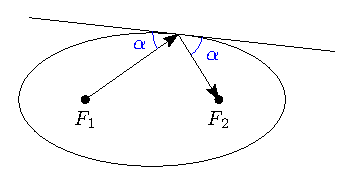
\includegraphics[width=0.3\textwidth]{ANGL2_1.eps}
	\caption{Оптические свойства эллипса.}
	\label{2_1}
\end{figure}
В школьной физике учат, что угол падения равен углу отражения

\uline{Геометрический смысл}: в точке касания (где находится касательная прямая) углы между отрезком из фокусов и касательной - равны. Тогда нам необходимо определить, что такое касательная прямая.

Если мы рассматрим эллипс и прямую, то возможны следующие взаимные расположения:
\begin{figure}[H]
	\begin{subfigure}[t]{.33\textwidth}
		\centering
		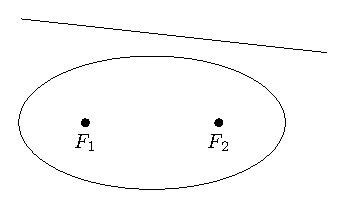
\includegraphics[width=0.9\textwidth]{ANGL2_2.eps}
		\caption{Точек пересечения нет.}
		\label{2_2}
	\end{subfigure}
	\begin{subfigure}[t]{.33\textwidth}
		\centering
		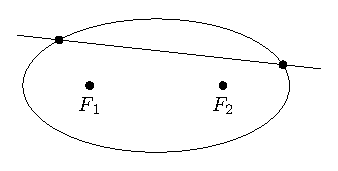
\includegraphics[width=0.9\textwidth]{ANGL2_3.eps}
		\caption{Прямая пересекает эллипс.}
		\label{2_3}
	\end{subfigure}
	\begin{subfigure}[t]{.33\textwidth}
		\centering
		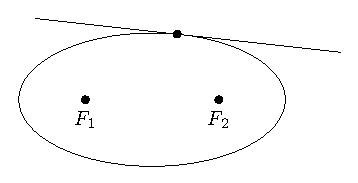
\includegraphics[width=0.9\textwidth]{ANGL2_4.eps}
		\caption{Прямая касается в одной точке.}
		\label{2_4}
	\end{subfigure}
	\caption{Взаимное расположение эллипса и прямой.}
\end{figure}
\begin{enumerate}[label=\arabic*)]
	\item Прямая не пересекает эллипс;
	\item Прямая пересекает эллипс в двух точках;
	\item Прямая пересекает эллипс по одной точке $\Rightarrow$ это касательная;
\end{enumerate}

\begin{rem}
	Больше, чем в двух точках прямая не может пересекать коническое сечение. Доказательство с помощью геометрической теории это сложная задача. С помощью аналитических методов это доказывается достаточно тривиально.
\end{rem}

\begin{defn}
	\uwave{Касательной прямой к конике} называется прямая, имеющая с коникой ровно одну точку, и в случае параболы - не параллельная  оси, а в случае гиперболы - не параллельная асимптотам.
\end{defn}
\begin{rem}
	Последнее замечание для параболы можно было бы убрать, используя проективную геометрию, поскольку парабола и прямая параллельная оси пересекались бы на бесконечности второй раз. Аналогично для гиперболы, мы уточням непараллельность асимптотам.
\end{rem}

\newpage
\begin{problem}[\textbf{\uline{Вспомогательная задача}}]
	Пусть две точки $A$ и $B$ лежат по одну сторону от прямой $l$. Как найти точку $X$ на прямой $l$, так, чтобы сумма расстояний $|AX| + |BX|$ была минимальной?
\end{problem}

\begin{rem}
	В анализе такая задача называется задачей условного экстремума.
\end{rem}
\begin{figure}[H]
	\centering
	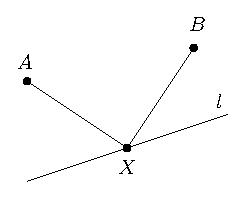
\includegraphics[width=0.2\textwidth]{ANGL2_5.eps}
	\caption{Поиск минимального: $|AX| + |BX|$.}
	\label{2_5}
\end{figure}
\begin{proof}
	Найдем точку $B'$ симметричную к $B$ относительно $l$. Проведём прямую $AB'$, тогда точка пересечения этой прямой с $l$ - будет искомой. Пусть есть некоторая точка $Y$, отличная от $X$.
	\begin{figure}[H]
		\centering
		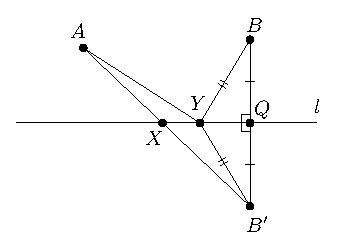
\includegraphics[width=0.3\textwidth]{ANGL2_6.eps}
		\caption{Доказательство минимальности точки $X$.}
		\label{2_6}
	\end{figure}
	Заметим, что в треугольники $BQY$ и $B'QY$ - равны, поскольку один катет - общий, а остальные равны по построению. Также заметим, что сторона $|AX|$ меньше, чем сумма двух других сторон по правилу треугольника. Тогда:
	$$
		|AY| + |BY| = |AY| + |B'Y| > |AX| + |B'X| = |AX| + |BX|
	$$
	Следовательно, точка $X$ - искомая.
\end{proof}

\begin{rem}
	Также заметим, что углы $\alpha$ равны как вертикальные, и если мы начертим прямую $BX$, то получающийся угол $\beta$ будет равен углу $\alpha$.
	\begin{figure}[H]
		\centering
		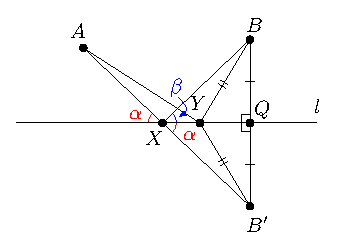
\includegraphics[width=0.3\textwidth]{ANGL2_7.eps}
		\caption{Закон отражения света.}
		\label{2_7}
	\end{figure}
\end{rem}

\begin{proof}
	Известно, что прямая делит плоскость на две полуплоскости, а если есть замкнутая непересекающаяся кривая, то она делит плоскость на две части, которая внутри этой кривой и которая вне этой кривой. Тоже самое происходит и с эллипсом. Пусть у нас есть эллипс с фокусами в точках $F_1$ и $F_2$, расстояние между которыми равно $2c$:
	$$
		|XF_1| + |XF_2| = 2a
	$$
	\begin{figure}[H]
		\centering
		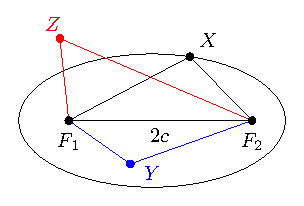
\includegraphics[width=0.25\textwidth]{ANGL2_8.eps}
		\caption{Оптические свойства эллипса.}
		\label{2_8}
	\end{figure}
	\begin{enumerate}[label=(\arabic*)]
		\item $|XF_1| + |XF_2| = 2a \Rightarrow X$ находится на эллипсе;
		\item $|YF_1| + |YF_2| < 2a \Rightarrow Y$ находится внутри эллипсе;
		\item $|ZF_1| + |ZF_2| > 2a \Rightarrow Z$ находится вне эллипсе;
	\end{enumerate}
	Если мы будем увеличивать $a$, то у нас будут растущие конфокальные эллипсы. И мы будем увеличивать $a$, пока не дойдем до нашего параметра, где будет касательная в точке $X$:
	$$
		|XF_1| + |XF_2| = 2a
	$$
	\begin{figure}[H]
		\centering
		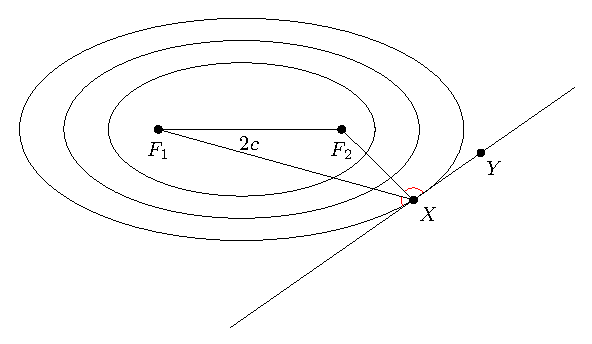
\includegraphics[width=0.5\textwidth]{ANGL2_9.eps}
		\caption{Увеличение параметра $a$.}
		\label{2_9}
	\end{figure}
	Если на этой касательной мы возьмем другую точку $Y$, которая лежит вне эллипса, то для неё:
	$$
		|YF_1| + |YF_2| > 2a
	$$
	Следовательно, $X$ - такая точка прямой, что сумма расстояний от $X$ до $F_1$ и $F_2$ - минимальна $\Rightarrow$ из вспомогательной задачи угол падения $=$ углу отражения. Таким образом, с точки зрения школьной геометрии мы доказали оптическое свойство эллипса.
	
\end{proof}

\begin{rem}
	Заметим, что это не совсем строго доказательство, но с точки зрения школьной геометрии вполне подходит.
\end{rem}

\subsection*{Гипербола}
\begin{rem}
	Оптическое свойство для гиперболы аналогично оптическому свойству эллипса и останется в качестве упражнения.
\end{rem}

\begin{prop}
	Луч выпущенный из одного фокуса после отражения движется так, будто он вышел из другого.
\end{prop}

\begin{figure}[H]
	\centering
	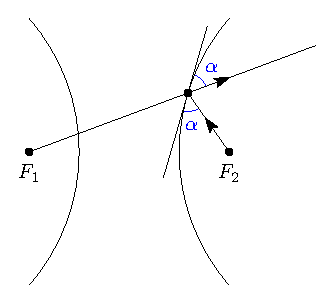
\includegraphics[width=0.3\textwidth]{ANGL2_10.eps}
	\caption{Оптические свойства гиперболы.}
	\label{2_10}
\end{figure}

Для гиперболы будет рассматриваться аналогичная вспомогательная задача, где будет требоваться найти максимальное расстояние между точками $A$ и $B$ по разную сторону прямой $l$.
\begin{figure}[H]
	\centering
	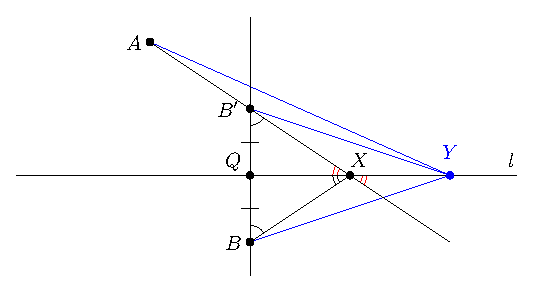
\includegraphics[width=0.5\textwidth]{ANGL2_11.eps}
	\caption{Вспомогательная задача для гиперболы.}
	\label{2_11}
\end{figure}
По аналогии, отзеркаливается точка $B$ до точки $B'$ и проводится прямая $AB'$. Точка пересечения этой прямой с прямой $l$ будет точка $X \Rightarrow$ в ней будет максимум разницы между $AX$ и $BX$, поскольку в любой другой точке на прямой $l$ будет работать правило треугольника. Аналогично из этой задачи найдем, что угол падения будет равен углу отражения: углы $BB'X$ и $B'BX$ будут равны, поскольку равны стороны, соответственно углы $BXQ$ и $B'XQ$ также будут равны, а угол отражения будет равен как вертикальный угол (на рисунке выделен красным).

\newpage
\subsection*{Парабола}
\begin{prop}
	Лучи выходящие из фокуса всегда будут параллельны оси параболы. Угол падения к касательной на параболе будет равен углу отражения от этой касательной.
\end{prop}

\begin{figure}[H]
	\centering
	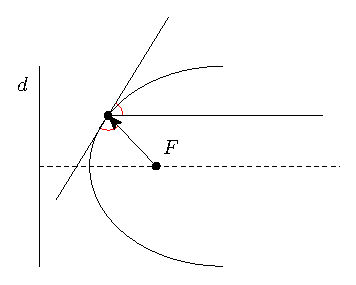
\includegraphics[width=0.3\textwidth]{ANGL2_12.eps}
	\caption{Оптические свойства параболы.}
	\label{2_12}
\end{figure}

\begin{proof}
	Пусть у нас задана парабола с фокусом в точке $F$ и директриссой $d$. Возьмем некоторую точку $X$, проведем линию $XF$ и опустим перпендикуляр $XY$ на директриссу. По определению:
	$$
		|XF| = |XY|
	$$
	Рассмотрим $YF$ и проведем к ней серединный перпендикуляр $l$, поскольку треугольник - равнобедренный, то он проходит через точку $X$. Докажем, что $l$ - касательная. Если $l$ была бы параллельна оси, то $YF$ была бы ортогональна этой оси и параллельна директриссе.

	\begin{figure}[H]
		\begin{subfigure}[t]{.5\textwidth}
			\centering
			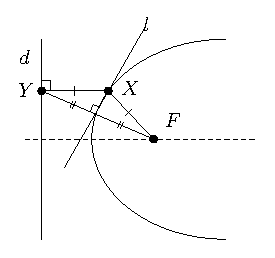
\includegraphics[width=0.5\textwidth]{ANGL2_13.eps}
			\caption{Построение касательной к параболе.}
			\label{2_13}
		\end{subfigure}
		\begin{subfigure}[t]{.5\textwidth}
			\centering
			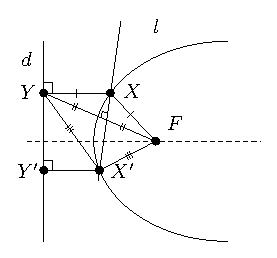
\includegraphics[width=0.5\textwidth]{ANGL2_14.eps}
			\caption{Построение $X'Y'$.}
			\label{2_14}
		\end{subfigure}
		\caption{Доказательство оптического свойства параболы.}
	\end{figure}
	Предположим, что $l$ пересекает параболу кроме $X$, ещё и в $X'$. Опустим из этой точки перпендикуляр $X'Y'$ на $d$. Поскольку $X'$ лежит на параболе, то:
	$$
		|X'Y'| = |X'F| 
	$$
	С другой стороны, $X'$ лежит на $l$, а поскольку $l$ - это серединный перпендикуляр, то:
	$$
		|X'F| = |X'Y| = |X'Y'| \Rightarrow Y' = Y
	$$
	где последнее верно в силу того, что перпендикуляр это кратчайшее расстояние до прямой, а $Y'$ это основание перпендикуляра. У параболы по основанию перпендикуляра однозначно восстанавливается точка: любая прямая, ортогональная директриссе пересекает параболу в одной точке, тогда: $X' = X$. Следовательно, $l$ - касательная.
	\begin{figure}[H]
		\centering
		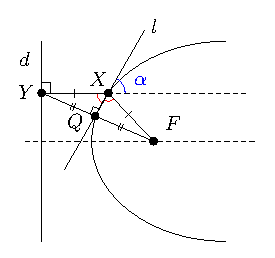
\includegraphics[width=0.25\textwidth]{ANGL2_15.eps}
		\caption{Доказательство равенства углов.}
		\label{2_15}
	\end{figure}
	Заметим, что $\triangle YXQ = \triangle XQF$, поскольку в равнобедренном треугольнике серединный перпендикуляр это и биссектриса, и медиана, и высота. Вместе с этим, по равенству вертикальных углов будет верно: 
	$$
		\angle YXA = \angle QXF = \angle \alpha
	$$
	Таким образом, угол падения $=$ углу отражения.
\end{proof}

\section*{Конфокальные коники}

\begin{defn}
	\uwave{Угол под которым пересекаются кривые} - угол между касательными к ним в точке пересечения.
\end{defn}

\begin{defn}
Коники называются \uwave{конфокальными}, если у них одинаковые фокусы.
\end{defn}
\begin{rem}
	В русской литературе ещё могут называться \textbf{софокусными} кониками.
\end{rem}

\begin{prop}
	Конфокальные эллипс и гипербола пересекаются под прямым углом.
\end{prop}
\begin{proof}
	Рассмотрим эллипс и гиперболу с одинаковыми фокусами.
	\begin{figure}[H]
		\centering
		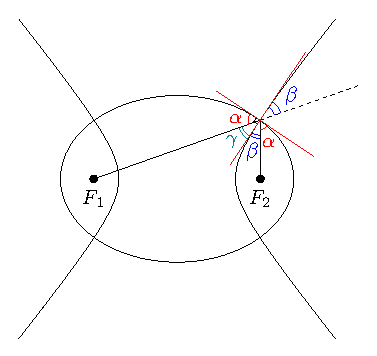
\includegraphics[width=0.35\textwidth]{ANGL2_16.eps}
		\caption{Пересечение эллипса и гиперболы.}
		\label{2_16}
	\end{figure}
	Из оптических свойств эллипса мы знаем про совпадение $\angle \alpha$, из оптических свойств гиперболы и равенства вертикальных углов мы знаем про совпадение $\angle \beta = \angle \gamma$, тогда:
	$$
		2\alpha + \beta + \gamma  = 2 \alpha + 2\beta = \pi \Rightarrow \alpha + \beta = \dfrac{\pi}{2}
	$$
	А поскольку $\alpha + \beta$ это угол между касательными, то они всегда ортогональны друг другу.
\end{proof}

Для параболы необходимо рассматривать параболы с общей осью и общим фокусом, но с разными директриссами, по разную сторону от фокуса. Параболы одного семейства не пересекаются, иначе у них будет общая точка и от неё расстояние до директриссы должно быть раво от этой точки  до фокуса, расстояние до фокуса одно $\Rightarrow$ и расстояние до директриссы одно $\Rightarrow$ эти параболы совпадают.
\begin{prop}
	Параболы с общей осью и фокусом или не пересекаются или пересекаются под прямым углом.
\end{prop}
\begin{proof}
	Рассмотрим разные семейства парабол. Из оптических свойств парабол, мы получим равенство углов падения и отражения, при проведении луча из фокуса до параболы: $\angle \alpha$ и $\angle \beta$.
	\begin{figure}[H]
		\centering
		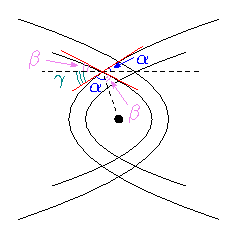
\includegraphics[width=0.25\textwidth]{ANGL2_17.eps}
		\caption{Пересечение парабол с разной директриссой.}
		\label{2_17}
	\end{figure}
	Поскольку отраженный лучи будут лежать на одной прямой (пересекающей точку пересечения парабол), то у нас будет равенство вертикальных углов: 
	$$
		\angle \gamma = \angle \alpha \Rightarrow 2\beta + \gamma + \alpha = 2\beta + 2\alpha= \pi \Rightarrow \alpha + \beta = \dfrac{\pi}{2}
	$$
	Таким образом, мы получили что $\alpha + \beta$ - это угол между касательными и они ортогональны друг другу.
\end{proof}

\newpage
\section*{Системы координат}
Из школы мы знаем, что координаты это что-то, где по паре чисел мы можем построить точку. Координаты не обязательно определены на всей плоскости, например, полярные координаты не определены в самом начале. Самая известная система координат - Декартова. 

Координатные линии получаются, если мы фиксируем одну координату и меняем другую. Например, если зафиксировать координату $x$ и менять $y$ или наоборот, то будут получаться вертикальные или горизонтальные линии соответственно.
\begin{figure}[H]
	\begin{subfigure}[t]{.5\textwidth}
		\centering
		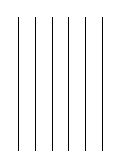
\includegraphics[width=0.2\textwidth]{ANGL2_18.eps}
		\caption{Фиксированная координата $x$, переменная $y$.}
		\label{2_18}
	\end{subfigure}
	\begin{subfigure}[t]{.5\textwidth}
		\centering
		
\includegraphics[width=0.3\textwidth]{ANGL2_19.eps}
		\caption{Фиксированная координата $y$, переменная $x$.}
		\label{2_19}
	\end{subfigure}
	\caption{Фиксирование координат.}
\end{figure}
Таким образом, получаем координатные кривые в Декартовых координатах, где координатные линии будут ортогональными.
\begin{figure}[H]
	\centering
	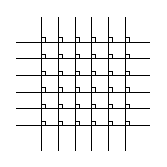
\includegraphics[width=0.2\textwidth]{ANGL2_20.eps}
	\caption{Координатные кривые в Декартовых координатах.}
	\label{2_20}
\end{figure}
Рассмотрим полярные координаты. Декартовы координаты задаются двумя осями, тогда как полярные координаты задаются точкой и лучом (длиной луча и углом поворота):
\begin{figure}[H]
	\centering
	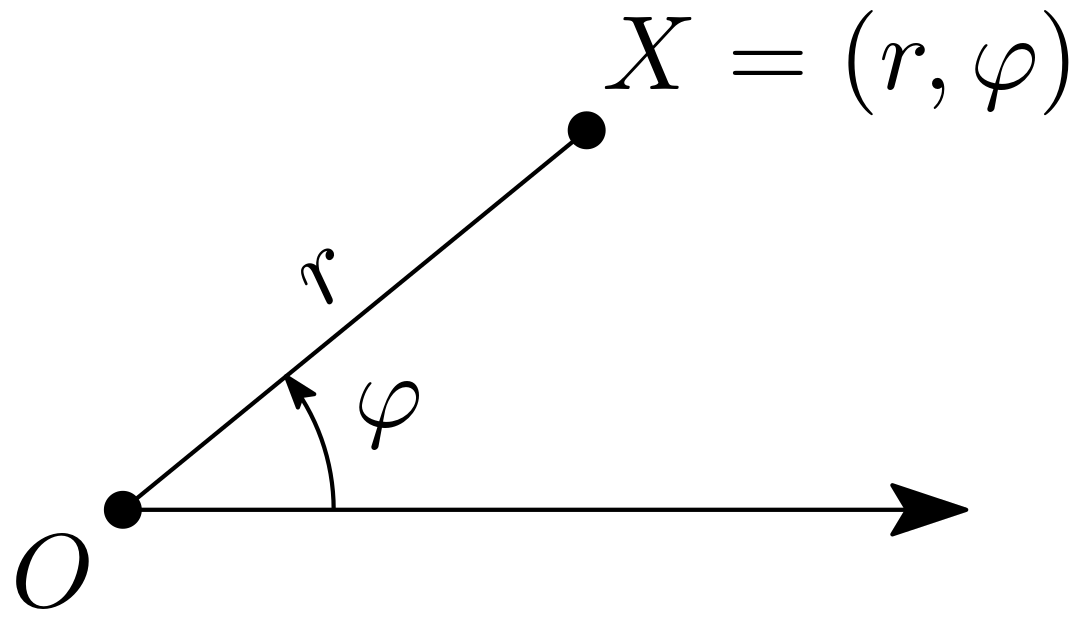
\includegraphics[width=0.2\textwidth]{ANGL2_21.png}
	\caption{Полярные координаты.}
	\label{2_21}
\end{figure}
\begin{rem}
	Заметим, что это не глобальные координаты, потому что у точки $O$ не определен угол.
\end{rem}
По аналогии с декартовыми координатами, если фиксируем радиус и меняем угол, то получаем окружности. Если фиксируем угол и меняем радиус, то получаем лучи. Следовательно, получаем координатные кривые для полярной системы координат. Также можно заметить, что радиусы ортогональны окружности.
\begin{figure}[H]
	\centering
	
\includegraphics[width=0.2\textwidth]{ANGL2_22.eps}
	\caption{Координатные кривые в полярной системе координат.}
	\label{2_22}
\end{figure}

По аналогии, с помощью софокусных эллипсов и гипербол, можно ввести эллиптические координаты. Для этого сначала фиксируются фокусы $F_1, F_2$. Затем координаты точки: $X = (a_1, a_2)$ задаются следующим образом:
$$
	|XF_1| + |XF_2| = 2a_1, \, ||XF_1| - |XF_2|| = 2a_2
$$
Поскольку фокусы заданы, то у нас есть единственный такой эллипс и единственная такая гипербола, и если мы находимся в первом квадранте, то такие координаты задают единственную точку.
\begin{figure}[H]
	\centering
	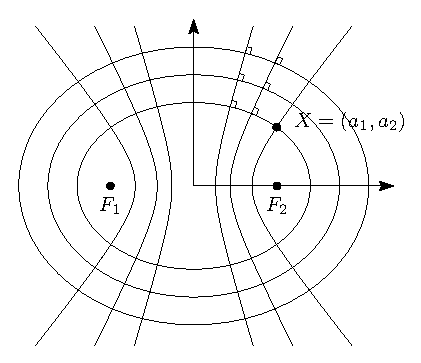
\includegraphics[width=0.35\textwidth]{ANGL2_23.eps}
	\caption{Эллиптические координаты.}
	\label{2_23}
\end{figure}
Координтнаые линии будут устроены так: если фиксируем фокусы и $a_1$, то получаем эллипсы, если фиксируем фокусы и $a_2$, то получаем гиперболы. Координатные линии также будут ортогональны.

\newpage
\section*{Аналитический подход}
Рассмотрев геометрический подход, мы можем отметить, что в рамках него все доказательства достаточно сложные. Некоторые факты доказать с помощью геометрического подхода было очень сложно (или даже практически невозможно в случае коник и кривых высоких порядков), поэтому дальнейшие продвижения в геометрии возникли с появлением аналитического метода Декарта.

\textbf{\uline{Аналитический подход Декарта}}: Необходимо точки заменять координатами этих точек, тогда всякие геометрические объекты заменяются уравнениями или неравенствами, которые эти геометрические объекты описывают.

\subsection*{Эллипс}
\begin{defn}
	\uwave{Эллипс} - это множество точек, координаты которых в некоторой ортогональной декартовой системе координат удовлетворяют уравнению:
	$$
		\dfrac{x^2}{a^2} + \dfrac{y^2}{b^2} = 1, \, a \geq b
	$$
\end{defn}

\begin{rem}
	Если $b = a$, то у нас было бы уроавнение окружности с радиусом $a$.
\end{rem}

Раньше, у нас было другое определение эллипса и нам нужно эти два определения сопоставить.
\begin{defn}
	\uwave{Эллипсом} называется геометрическое место точек (то есть, множество), таких, что сумма расстояний от них до двух фиксированных точек (называемых \uwave{фокусами эллипса}) постоянна.
\end{defn}
\begin{prop}
	Алгебраическое и геометрическое определения эллипса эквивалентны.
\end{prop}
\begin{proof}
	Пусть $F_1, F_2$ - фокусы, тогда мы смотрим на множество точек $X$ таких, что:
	$$
		|XF_1| + |XF_2| = 2a
	$$
	\begin{figure}[H]
		\centering
		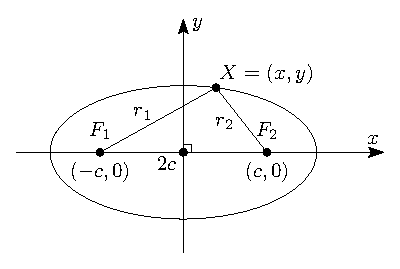
\includegraphics[width=0.35\textwidth]{ANGL2_24.eps}
		\caption{Связь аналитического и геометрического определения эллипса.}
		\label{2_24}
	\end{figure}
	\begin{rem}
		В аналитической геометрии по возможности надо стараться выбирать координаты так, чтобы всё было симметричным. Например, эллипс задается через две точки $\Rightarrow$ обязательно выбирайте начало координат в центре отрезка между этими двумя точками (в данном случае, в центре отрезка $F_1F_2$). Оси также выбираем ортогонально.
	\end{rem}
	Таким образом, зададим следующие обозначения:
	$$
		F_1 = (-c,0), \, F_2 = (c, 0), \, X = (x,y), \, |F_1 X| = r_1, \, |F_2 X| = r_2
	$$
	Расстояние между точками найдем как в школе и подставим в геометрическое уравнение эллипса:
	$$
		r_1 = \sqrt{(x + c)^2 + (y - 0)^2}, \, r_2 = \sqrt{(x - c)^2 + (y - 0)^2} \Rightarrow |XF_1| + |XF_2| = 2a
	$$
	Далее, проведём элементарные преобразования:
	$$
		\sqrt{(x + c)^2 + y^2} + \sqrt{(x - c)^2 + y^2} = 2a \Rightarrow \sqrt{(x + c)^2 + y^2}   = 2a - \sqrt{(x - c)^2 + y^2} \Rightarrow
	$$
	$$
		\Rightarrow (x+c)^2 + y^2 = 4a^2 + (x-c)^2 + y^2 - 4a\sqrt{(x - c)^2 + y^2} \Rightarrow 4a\sqrt{(x - c)^2 + y^2} = 4a^2 - 4xc \Rightarrow
	$$
	$$
		\Rightarrow a\sqrt{(x - c)^2 + y^2} = a^2 - xc \Rightarrow a^2(x-c)^2 +a^2y^2 = a^4 + x^2c^2 - 2a^2xc \Rightarrow
	$$
	$$
		\Rightarrow (a^2 - c^2)x^2 + a^2y^2 = a^4 - a^2c^2 \Rightarrow \dfrac{x^2}{a^2} + \dfrac{y^2}{a^2 - c^2} = 1 
	$$
	Получаем аналитическое уравнение для: 
	$$
		b = \sqrt{a^2 - c^2}
	$$ 
	Поскольку $a > c$ (когда определяли эллипс, иначе множество - бессмысленное), то: $b > 0$. Также заметим, что $b \leq a$, где равенство возможно в случае, когда $c = 0$ (окружность). Таким образом, у геометрического эллипса в выбранной системе координат координаты точек удовлетворяют аналитическому уравненияю с $b = \sqrt{a^2 - c^2}$.
	
	\begin{rem}
		Заметим, что мы не доказали, что получим все точки, удовлетворяющие аналитическому уравнению (поскольку совершали операции возведения в квадрат, например).
	\end{rem}
	
	Необходимо доказать, что все точки, удовлетворяющие аналитическому уравнению лежат на геометрическом эллипсе. Введем: $c, F_1, F_2$ такие, что:
	$$
		c = \sqrt{a^2 - b^2}, \, F_1 = (-c, 0), \, F_2 = (c,0)
	$$
	Пусть $X = (x,y)$ и $X$ удовлетворяет аналитическому уравнению. Найдем $r_1 = |XF_1|$ и $r_2 = |XF_2|$:
	$$
		r_1 = \sqrt{(x + c)^2 + (y - 0)^2}, \, \dfrac{x^2}{a^2} + \dfrac{y^2}{b^2} = 1 \Rightarrow y^2 = b^2 - \dfrac{b^2}{a^2}x^2 \Rightarrow 
	$$
	$$
		\Rightarrow r_1 = \sqrt{(x+c)^2 + b^2 - \dfrac{b^2}{a^2}x^2} = \sqrt{x^2 + 2xc + c^2 + a^2 - c^2 - \dfrac{a^2 - c^2}{a^2}x^2} = 
	$$
	$$
		= \sqrt{\dfrac{c^2}{a^2}x^2 + 2xc + a^2} = \sqrt{\left(a + \dfrac{c}{a}x\right)^2}
	$$
	Из аналитического уравнения видим, что сумма слагаемых равна $1 \Rightarrow$ каждое из слагаемых не больше, чем $1$, тогда будут верны неравенства: 
	$$
		|x| \leq a \wedge |y| \leq b
	$$ 
	Этот прямоугольник называется \uwave{основным прямоугольником эллипса}.
	
	\begin{exrc}
		Доказать, что:
		$$
			a + \dfrac{\sqrt{a^2 - b^2}}{a}x \geq 0
		$$
	\end{exrc}
	\begin{proof}
		$$
			a \geq b > 0, \, |x| \leq a \Rightarrow a + \dfrac{x}{a}{\cdot}\sqrt{a^2 - b^2} \geq a - \sqrt{a^2 - b^2} \geq 0
		$$
	\end{proof}
	Из доказанного выше, мы получаем:
	$$
		a + \dfrac{\sqrt{a^2 - b^2}}{a}x \geq 0\Rightarrow r_1= a + \dfrac{c}{a}x
	$$
	Аналогичное вычисление для $r_2$, тогда:
	$$
		|XF_1| + |XF_2| = r_1 + r_2 = a + \dfrac{c}{a}x + a - \dfrac{c}{a}x = 2a
	$$
	Таким образом, если точка удовлетворяет аналитическому уравнению, то она лежит на геометрическом эллипсе. Следовательно, геометрическое и аналитическое определения - одинаковы.
\end{proof}


\end{document}